\documentclass[12pt]{article}

\usepackage[a4paper, margin=1in]{geometry}
\usepackage{xcolor}
\usepackage{amsmath}
\usepackage{tcolorbox}
\usepackage{tikz}
\usetikzlibrary{arrows.meta,positioning}
\usepackage{fontawesome5} % icons
\usepackage{hyperref}
\usepackage{graphicx}
\usepackage{float}
\usepackage{comment}
\usepackage[nameinlink,capitalize,noabbrev]{cleveref}
\usepackage{subcaption} % modern replacement for the deprecated subfigure package

\setlength{\parindent}{0pt}

% === COLOR PALETTE (customize these) ===
\definecolor{maincolor}{HTML}{2A9D8F} % your teal
\definecolor{accentcolor}{HTML}{E76F51}
\definecolor{lightcolor}{HTML}{FFDEAD}

% Tell cleveref how to name your counter
\crefname{exercise}{assignment}{assignments}
\Crefname{exercise}{Assignment}{Assignments}

% === ASSIGNMENT STYLE ===
\newcounter{exercise}

% Optional label: \exercisetitle[<label>]{<Title>}
\newcommand{\exercisetitle}[2][]{%
  \refstepcounter{exercise}% make this step referenceable/hyperlinked
  \vspace{0.5cm}%
  \colorbox{maincolor}{%
    \makebox[\dimexpr\linewidth-2\fboxsep][l]{%
      \textcolor{white}{\faPen\ Assignment \theexercise:~ #2}%
    }%
  }%
  % If an optional label was provided, set it
  \if\relax\detokenize{#1}\relax\else\label{#1}\fi
  \vspace{0.3cm}%
}


% === IMPORTANT BOX ===
\newtcolorbox{importantbox}{
  colback=lightcolor,
  colframe=accentcolor,
  arc=4mm,
  boxrule=1pt,
  left=6pt,
  right=6pt,
  top=6pt,
  bottom=6pt
}

% === PROMPT BOX ===
\newtcolorbox{promptbox}{
  colback=white,
  colframe=maincolor,
  arc=4mm,
  boxrule=1pt,
  left=6pt,
  right=6pt,
  top=6pt,
  bottom=6pt
}

% === QUESTION BOX (with starred variant and cleveref names) ===
% Requires: \usepackage{hyperref} for \Form/\TextField
%           \usepackage{fontawesome5} for \faEdit

% Cleveref names for the question counter
\crefname{question}{question}{questions}
\Crefname{question}{Question}{Questions}

\makeatletter
\newcounter{question}
\newlength\questionheight
\setlength\questionheight{5cm} % default answer box height

% \question{<text>}                  -> with TextField (default height)
% \question[<height>]{<text>}        -> with TextField (custom height)
% \question*{<text>}                 -> no TextField, still numbered
\newcommand{\question}{\@ifstar{\question@text}{\question@field}}

% Common heading (increments counter and creates ref anchor)
\newcommand{\question@heading}[1]{%
  \refstepcounter{question}%
  \vspace{0.3cm}%
  \noindent\textbf{\faEdit\ Question \thequestion: #1}%\\[0.3em]%
}

% Starred form: numbered question without input field
\newcommand{\question@text}[1]{%
  \question@heading{#1}%
%  \vspace{0.3cm}%
}

% Unstarred form: numbered question with input field (optional height)
\newcommand{\question@field}[2][\questionheight]{%
  \question@heading{#2}%
 \\[0.3em] \begin{Form}
    \TextField[
      name=Q\thequestion,
      multiline=true,
      width=\linewidth,
      height=#1,
      charsize=10pt,
      bordercolor={0 0 0},
      borderwidth=1.8,
      backgroundcolor={1 1 1}
    ]{}
  \end{Form}
  \vspace{0.3cm}%
}
\makeatother

% === SOLUTION BOX ===
% Definition of solution/no solution environment for teacher and student versions

% === Teacher toggle ===
\newif\ifteacher
\teacherfalse% Write teacherfalse for student version and teachertrue for teachers version

% === Solution environment ===
\newtcolorbox{solutionbox}{colback=gray!10,colframe=black!60!black,arc=1mm,boxrule=1pt}

\ifteacher
\newenvironment{solution}{%
  \begin{solutionbox}\textbf{Solution:}
}{%
  \end{solutionbox}
}
\else
  \excludecomment{solution}
\fi

% === CALCULATION / ANSWER SPACE (printable AND fillable as PDF form fields) ===
\newcounter{answerfield}
% \calcspace[<height>] : a multiline box to write calculations in; fillable in a PDF viewer
\newcommand{\calcspace}[1][4cm]{%
  \par\vspace{2pt}%
  \refstepcounter{answerfield}%
  \begin{Form}
    \TextField[
      name=F\theanswerfield,
      multiline=true,
      width=\linewidth,
      height=#1,
      charsize=10pt,
      bordercolor={0 0 0},
      borderwidth=1,
      backgroundcolor={1 1 1}
    ]{}
  \end{Form}%
  \par\vspace{4pt}%
}
% \answerbox[<width>]{<label>} : an inline fill-in field, e.g. \answerbox{$MSE ={}$}
\newcommand{\answerbox}[2][3cm]{%
  \refstepcounter{answerfield}%
  #2~\begin{Form}\TextField[
      name=F\theanswerfield,
      multiline=false,
      width=#1,
      height=1.1em,
      charsize=10pt,
      bordercolor={0 0 0},
      borderwidth=1,
      backgroundcolor={1 1 1}
    ]{}\end{Form}%
}

\begin{document}

\begin{titlepage}

% === Top spacing ===
\vspace*{1cm}

% --- Project logo ---
\begin{center}
    
\includegraphics[height=3cm]{Figures/Logo_TAI_Transparent.png}
\end{center}

\vspace{0.8cm}

% === Title page ===
\begin{center}
    {\Huge \bfseries \color{maincolor} Fitting and machine learning\par}
    \vspace{0.5cm}
    
    {\Large \color{accentcolor} Teaching with AI (TAI) \par}
    
    \vspace{1.5cm}
    
    \begin{center}
{\large
Mirte van der Eyden$^{1}$, Andrea López Incera$^{2}$ \\[0.3cm]

{\small
$^{1}$ Institut für Fachdidaktik, Universität Innsbruck \\ 
mirte.van-der-eyden@uibk.ac.at \\[0.2cm]


$^{2}$ Departament de didàctica de la matemàtica i les ciències experimentals, Universitat Autònoma de Barcelona \\ 
andrea.lopez.incera@uab.cat
}
}
\end{center}

\end{center}

\vfill

% === Logos at the bottom ===
\begin{center}
\begin{tabular}{cccc}

\includegraphics[height=1.5cm]{Figures/Logos/universitaet-innsbruck-logo-cmyk-farbe.jpg} &

\includegraphics[height=1.5cm]{Figures/Logos/logotipuab-v1-verd.png} &

\includegraphics[height=1.5cm]{Figures/Logos/EN Co-funded by the EU_POS.jpg} \\

\includegraphics[height=1.5cm]{Figures/Logos/IMG_1189.PNG} &

\includegraphics[height=1.8cm] {Figures/Logos/2nd Lyceum of Kos logo.jpg} &

\includegraphics[height=1.5cm]{Figures/Logos/NEXT_prov_logo.png}
\end{tabular}
\end{center}


\vspace{0.5cm}

% Optional footer text
\begin{center}
    {\small Project funded by Erasmus+ Programme of the European Union}
\end{center}

\end{titlepage}

% === Description of activity ===
\vspace*{0.2\textheight}

Subject: Mathematics


\vspace{0.3cm}

Activity duration: 165 min, split over two sessions of 90 and 75 minutes (break after step 3).

\vspace{0.5cm}

Steps:
\begin{enumerate}
    \item Intro and connection to exoplanets (15 min)
    \item Linear regression and loss functions (45 min)
    \item Fitting functions (30 min)
    \item Neural networks presentation (10 min)
    \item Working with a neural network (40 min)
    \item Discover Kepler's Law (15 min)
    \item Application to exoplanet (10 min)
\end{enumerate}

\vspace{0.1cm}
The first session (steps 1--3) takes 90 minutes; the second session (steps 4--7) takes 75 minutes.

Learning goals:

\begin{itemize}
    \item Modelling a relationship in data with a function, and fitting it by tuning parameters
    \item Loss functions and the mean squared error (MSE)
    \item Linear regression, and finding the optimal fit by minimising the loss (by reasoning, by calculus, and the idea behind gradient descent)
    \item Comparing different models (linear, quadratic, power law) and choosing the best one
    \item Training and testing data, and why a model must generalise
    \item What machine learning and neural networks are, and how they are trained
    \item Interpretable models versus flexible ``black-box'' models, and when to use each type
    \item Using Python (and, optionally, an AI assistant) to fit models, and checking the results critically
    \item Rediscovering Kepler's third law from data, and using it to find an exoplanet's orbit
\end{itemize}

\newpage

% === HEADER / BRANDING ===
\begin{center}
    {\LARGE \color{maincolor} Fitting and machine learning}\\[5pt]
    {\large \textit{A mathematics lesson about AI}}\\
    \rule{\linewidth}{1pt}
\end{center}

\vspace{0.5cm}

\textit{In this lesson, we follow in the footsteps of Johannes Kepler. Starting with a table of planetary data, we learn how to fit mathematical models, measure how well they describe the data, and explore how machine learning and neural networks find patterns. We also consider when these methods are useful and when a simpler model is preferable. Along the way, we rediscover one of the most famous laws in astronomy and use it to determine the orbit of an exoplanet.}

\vspace{0.3cm}

\section{Introduction}

An exoplanet's orbital period can be determined from its transit light curve. The orbital period is the time the planet takes to complete one orbit around its star. Earth's orbital period is one year, whereas known exoplanets have periods ranging from a few hours to many years.

The orbital period can reveal further information about a planet's orbit. In this lesson, you will learn how to estimate the size of a planetary orbit from its period.

Planets move in elliptical orbits around their host stars (\cref{fig:ellipse}). Johannes Kepler discovered this in the early 17th century, before Newton developed his laws of motion and universal gravitation. Kepler analysed Tycho Brahe's precise observations of planetary positions and concluded that the planets follow elliptical rather than circular paths.

Because an orbit is elliptical, the planet's distance from its star changes throughout the orbit. When astronomers describe the size of an orbit, they usually use its \emph{semi-major axis}. This distance is indicated in \cref{fig:ellipse}.
\begin{figure}[htbp]
    \centering
    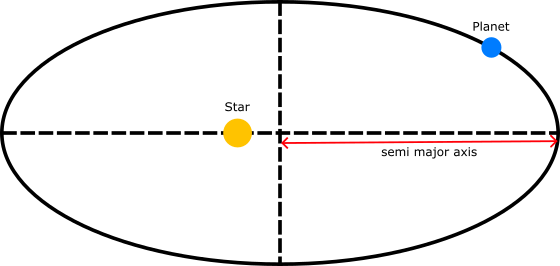
\includegraphics[width=0.5\linewidth]{Figures/math/ellipse.png}
    \caption{An elliptical planetary orbit with the semi-major axis indicated in red.}
    \label{fig:ellipse}
\end{figure}

\vspace{0.5cm}
\textcolor{accentcolor}{\textbf{\faLightbulb\ Initial ideas}}

\question{Why is it interesting to know the distance from an exoplanet to its star?}

\question[3cm]{Can a planet orbit its host star at any speed? Explain your reasoning.}

\question[3cm]{Do you expect a relationship between an exoplanet's orbital period and the semi-major axis of its orbit? If so, what relationship do you predict, and why?}

To test whether such a relationship exists, we need observations of planets for which both the orbital period and the semi-major axis are known. We therefore begin with the planetary system closest to us: the Solar System. Because its planets are relatively nearby, astronomers can determine their positions, orbital periods, and distances using several observational methods. Tycho Brahe made exceptionally precise measurements of planetary positions in the late 16th century. The orbital periods and semi-major axes of the Solar System planets are shown in \cref{fig:solarsystem}.

\begin{figure}[htbp]
    \centering
    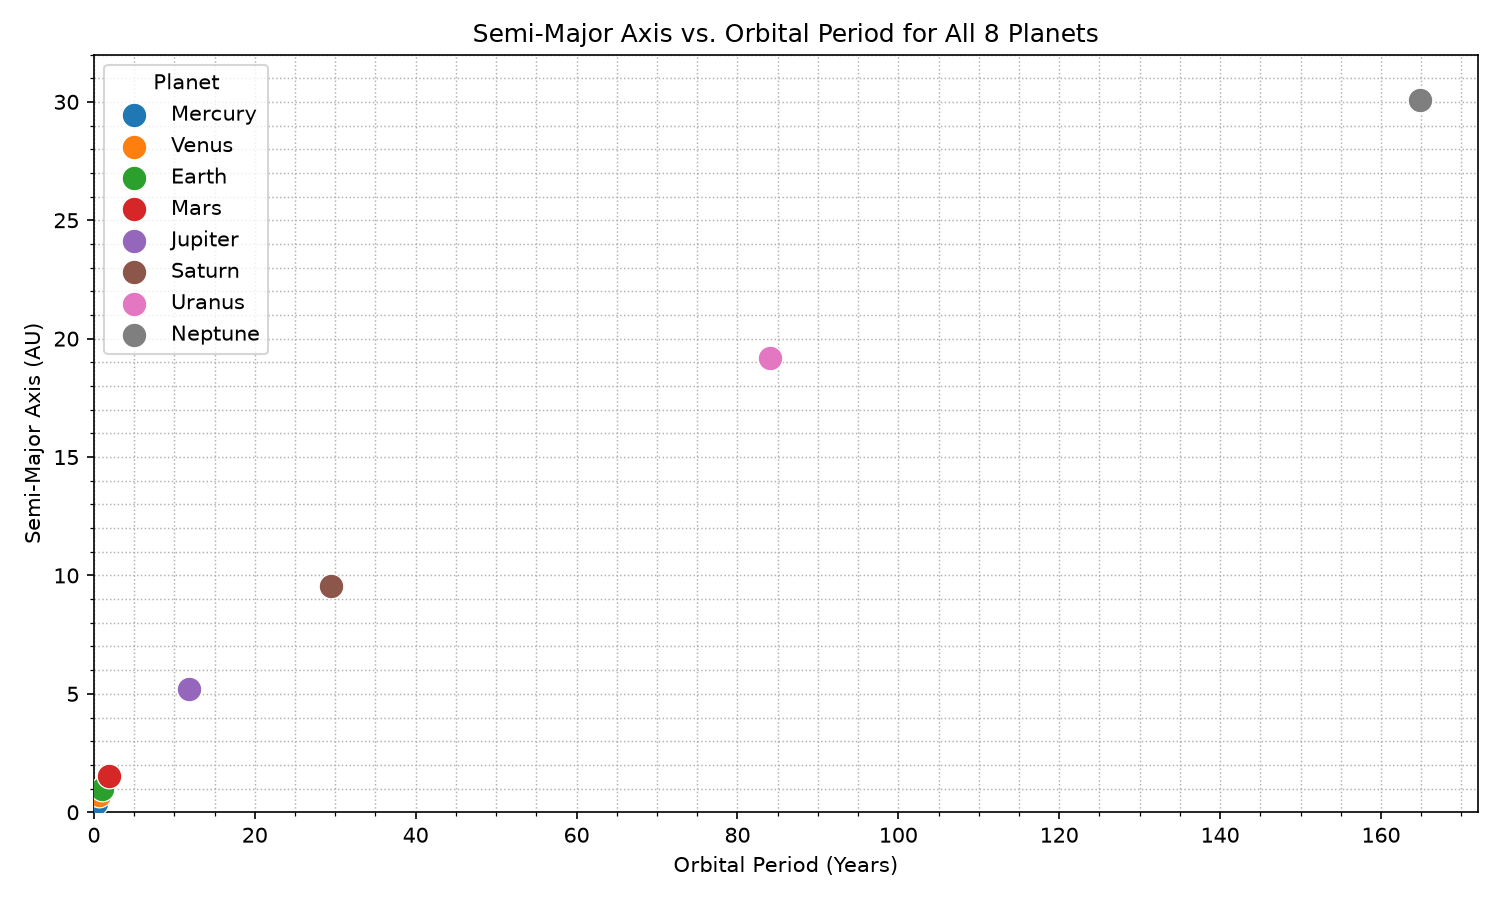
\includegraphics[width=0.95\linewidth]{Figures/math/all_planets_intro.png}
    \caption{Orbital periods and semi-major axes of the planets in the Solar System.}
    \label{fig:solarsystem}
\end{figure}

Kepler studied Brahe's data and found a mathematical relationship between orbital period and orbital size. He formulated this relationship as what we now call \emph{Kepler's third law}. Kepler lived before Newton and therefore did not know the law of universal gravitation. Although Kepler's physical explanation for planetary motion was incorrect, the mathematical pattern he identified in the data was accurate.

Today, we follow in Kepler's footsteps and try to discover the relationship between orbital period and semi-major axis directly from the data. We also have tools that Kepler did not: computers, neural networks, and other machine-learning methods. How can machine learning help us find relationships in data, and what limitations does it have?

\vspace{0.5cm}
\textcolor{accentcolor}{\textbf{\faLightbulb\ The Challenge}}

\begin{importantbox}
\textbf{Challenge:} Discover the relationship between planetary orbital period and semi-major axis, then use it to estimate the distance between your exoplanet and its star.
\end{importantbox}

To complete this challenge, you will work through the following steps:

\begin{enumerate}
    \item Fit and compare several possible relationships, including linear, quadratic, and power-law models.
    \item Explore the basic ideas behind machine learning and neural networks.
    \item Rediscover Kepler's third law and apply it to an exoplanet.
\end{enumerate}

\vspace{0.5cm}
\textcolor{accentcolor}{\textbf{\faLightbulb\ Constructing new ideas}}

\section{Linear regression and loss functions}\label{sec:linreg}

To find a relationship in the data, we describe it with a \emph{model}: a mathematical function that takes an input (here, the orbital period $T$) and returns a prediction for an output (here, the semi-major axis $a$). A model has one or more \emph{parameters}: numbers that we are free to choose. \emph{Fitting} a model means adjusting these parameters until the model matches the data as closely as possible.

The simplest relationship we can try is a \emph{linear} one: a straight line. In this section, we fit a straight line to data from the inner planets, define what it means for a fit to be ``good'', and find the best possible line. Along the way, we encounter two ideas that lie at the heart of machine learning: the \emph{loss function} and the distinction between \emph{training data} and \emph{testing data}.

\exercisetitle{Finding the best fit}

The graph shows orbital period versus distance for the four planets closest to the Sun.
\begin{figure}[htbp]
    \centering
    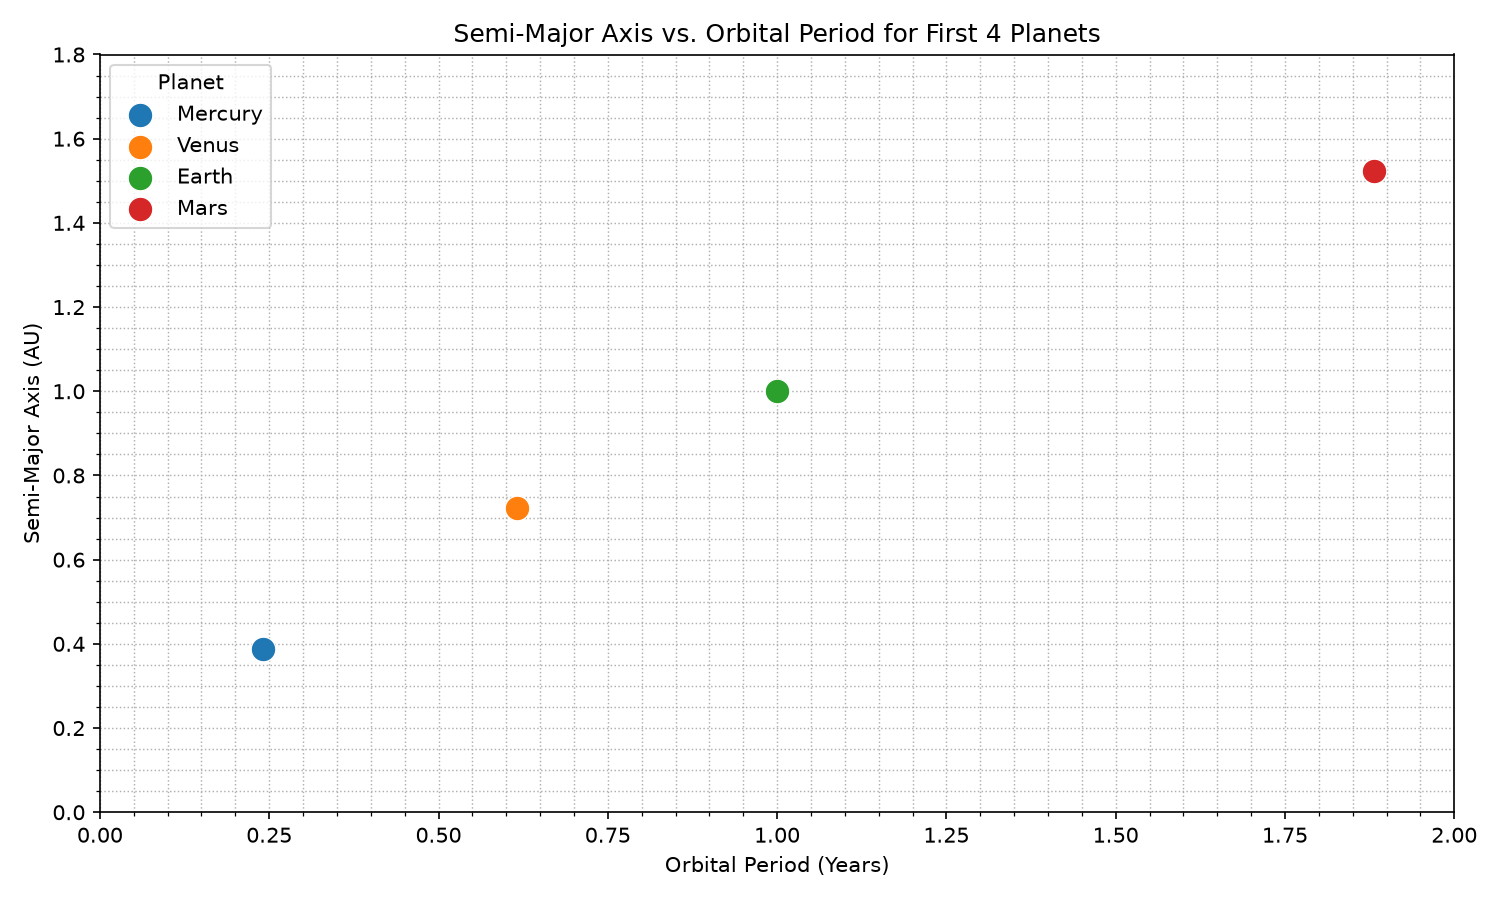
\includegraphics[width=0.95\linewidth]{Figures/math/4_planets_3.png}
    \caption{Orbital period and semi-major axis of the four inner planets in the Solar System.}
    \label{fig:4_planets}
\end{figure}

The exact data values are given in the table below.

\vspace{0.5cm}
\begin{tabular}{|c|c|c|}
\hline
  Planet & Orbital period (years)   & Semi-major axis (AU)  \\ \hline
   Mercury  & 0.240847	& 0.387099  \\ \hline
   Venus& 0.615197	& 0.723332  \\ \hline
   Earth& 1.000017	& 1.000000  \\ \hline
   Mars& 1.880816	& 1.523662  \\ \hline
\end{tabular}
\vspace{0.5cm}

Remember that our goal is to predict a planet's orbital size (its semi-major axis $a$) from its orbital period $T$. We therefore treat $T$ as the input and place it on the horizontal axis, while $a$ is the output and appears on the vertical axis.

\question{Describe the relationship you see in the data.}
\question{Could this relationship be linear? What would a linear model look like on the graph?}

To learn how fitting works, we start with a linear fit. For the simplest version of a linear fit, we require the line to pass through the origin. We use a model of the form $y = cx$, where $x$ is the orbital period $T$, $y$ is the semi-major axis $a$, and $c$ is the single adjustable parameter: the slope.

\textcolor{maincolor}{\textbf{\faPen\ a) Draw a linear fit through the four data points.}}

\question{How good is this fit? Do you think this captures the relation between the points?}

\question{How would you quantify how good this fit is?}

We define a function, called the \emph{Loss function (L)}, that quantifies how far our model/fit is away from the actual data points. Naively, it comes down to calculating how far the points in your plot are distanced from the line that you drew. As modellers, we have to choose how exactly to define our loss function. 

In this lesson, we choose to calculate the loss function with the \emph{mean squared error (MSE)}. This can be calculated with the following steps: 

\begin{enumerate}
    \item For every data point $(x_i,y_i)$ that you have, you draw the point $(x_i,\hat{y}_i)$ that lies on the fitting line. 
    \item For every data point, measure the difference between $y_i$ and $\hat{y}_i$. This is the difference between where your data point is, and where your model predicts it to be and is called the \emph{error}. 
    \item Calculate the \emph{square} of this error for every data point. 
    \item Calculate the \emph{mean} value of these squares, over all data points. 
\end{enumerate}
Together this forms the following formula for the \emph{mean square error (MSE)}:
$$MSE = \frac{1}{n}\sum_i^n (y_i - \hat{y}_i)^2.$$

We define our loss function to be the mean square error. $$ L = MSE.$$

\textcolor{maincolor}{\textbf{\faPen\ b) Calculate the $MSE$ for your fit.}} Use the space below for your calculation.

\calcspace[5cm]

\answerbox{$MSE ={}$}

\question{How satisfied are you with your fit? Do you think this is the most optimal fit possible?}

We want to find the \emph{optimal} fit: the one for which the $MSE$ is as low as possible. There are two different ways to reach it. Choose the route that matches what you have learned so far. You only need to do \emph{one} of them.

\begin{importantbox}
\textbf{Choose your route:}
\begin{itemize}
  \item \textbf{Route 1: Optimize by hand.} If you have \emph{not} learned how to differentiate yet, follow Route~1. You will improve your fit by hand and reason about how to find the very best one.
  \item \textbf{Route 2: Optimize with calculus.} If you \emph{do} know how to differentiate, skip Route~1 and go straight to Route~2, where you compute the optimal fit exactly.
\end{itemize}
\end{importantbox}

\subsection*{Route 1: Optimize by hand}

To find a better fit, it helps to compare your fit with another one. On the graph below you can draw a second attempt.

\begin{figure}[htbp]
    \centering
    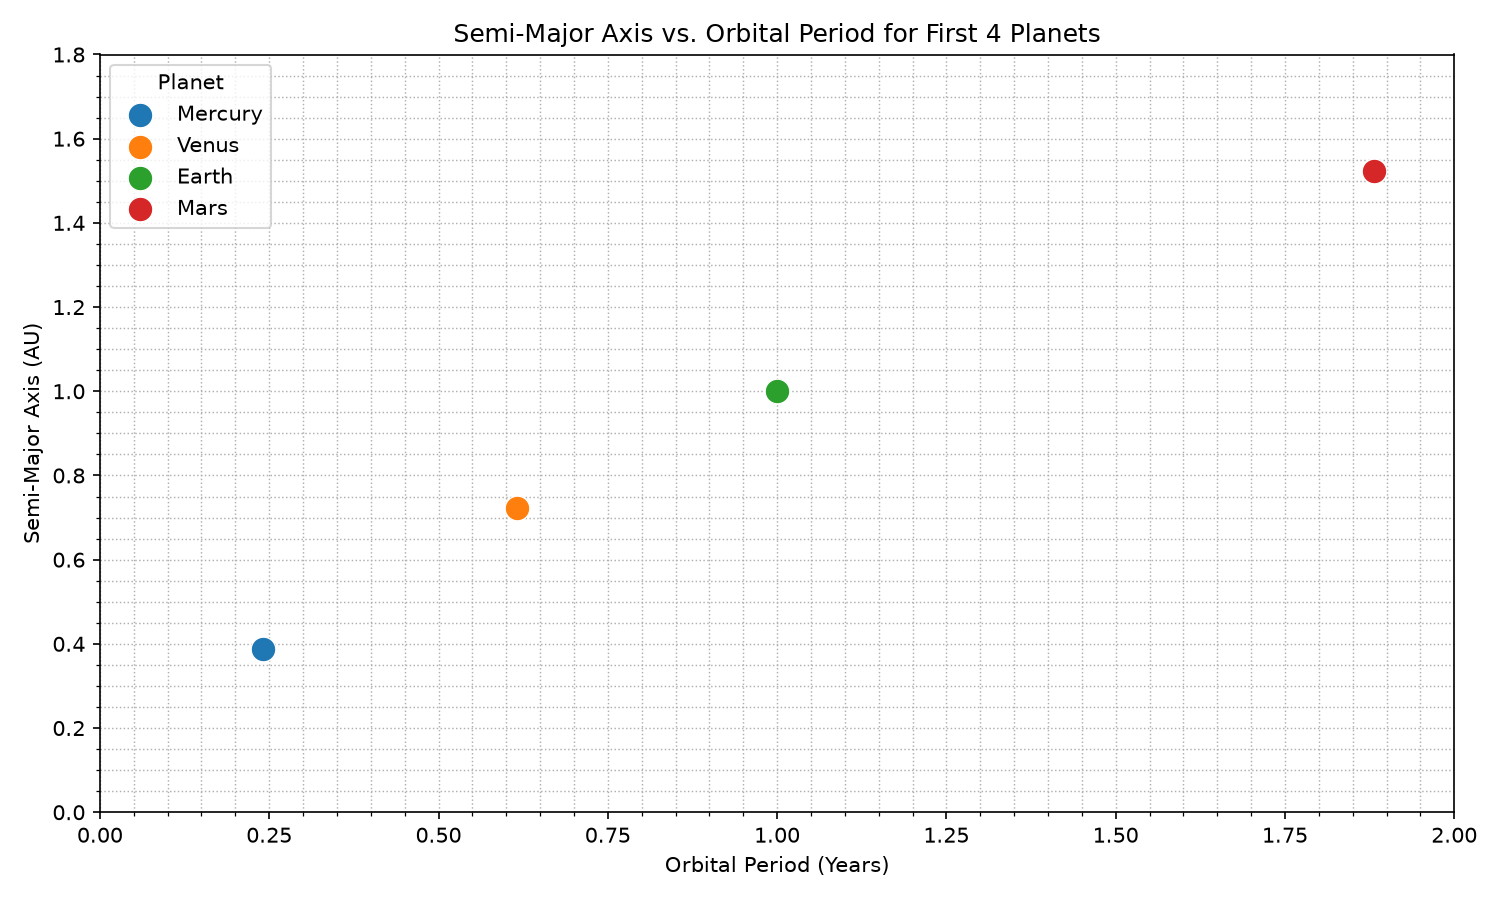
\includegraphics[width=0.95\linewidth]{Figures/math/4_planets_3.png}
    \caption{Period and semi major axis of the first four planets in our solar system.}
    \label{fig:4_planets_route1}
\end{figure}

\textcolor{maincolor}{\textbf{\faPen\ c) Draw another possible fit and again calculate the $MSE$.}} Make it really different. If you did not manage to improve on your previous fit, draw any other (possibly worse) option and still calculate the $MSE$.

\calcspace[4cm]

\question[1cm]{Which fit was better?}

Both fits you drew have the form $\hat{y}=cx$. The value of $c$ completely determines the fit.

\textcolor{maincolor}{\textbf{\faPen\ d) Determine the slope $c$ of each of your two attempts, and complete the table below with each value of $c$ and its corresponding $MSE$.}}

\vspace{0.5cm}
\begin{tabular}{|c|c|}
\hline
    $c$ & $MSE$ \\ \hline
     &  \\ \hline
     &  \\ \hline
\end{tabular}
\vspace{0.5cm}

For every value of $c$ we get a different value of $MSE$. Finding the best fit means finding the $c$ for which the $MSE$ is lowest. You are now going to reason about how to get there step by step, without any advanced mathematics.

\question[3cm]{Look at your table. As you change $c$, what happens to the $MSE$? Does it always change in the same direction?}

\question[4cm]{Suppose you compute the $MSE$ for your value of $c$, and then again for a slightly \emph{larger} $c$. How does comparing these two values tell you whether you should increase or decrease $c$ to lower the $MSE$?}

\question[6cm]{Describe a step-by-step procedure that starts from any guess for $c$ and gets closer and closer to the best value, using only your ability to compute the $MSE$. How would you decide in which direction to step, how big your steps should be, and when to stop?}

\begin{solution}
This is exactly the idea behind \emph{gradient descent}, the method used to train most machine learning models. Starting from a guess for $c$: (1) compute the $MSE$; (2) test a nearby value to find out whether increasing or decreasing $c$ lowers the $MSE$, thereby estimating the slope (gradient) of the $MSE$ curve; (3) take a step in the direction that lowers the $MSE$; and (4) repeat. The steps should get smaller as you approach the minimum, and you stop when the $MSE$ no longer decreases. Route~2 finds this same minimum exactly using differentiation.
\end{solution}

\textcolor{maincolor}{\textbf{\faPen\ e) Using this reasoning, find the best value of $c$ you can by hand, and write down your best model.}}

\answerbox[5cm]{$\hat{y} ={}$}

\medskip
\emph{Route~1 is complete. Continue at ``Testing the model'' below.}

\subsection*{Route 2: Optimize with calculus}

Instead of guessing, we can find the optimal $c$ exactly. We treat the $MSE$ as a function of $c$ and look for the minimum of that function.

Recall that the $MSE$ is
$$MSE = \frac{1}{n}\sum_i^n (y_i - \hat{y}_i)^2,$$
and that our linear model predicts $\hat{y}_i = c\,x_i$.

\question[3.5cm]{Substitute $\hat{y}_i = c\,x_i$ into the formula above, to write the $MSE$ as a function of $c$. Then draw a circle around every $c$ that appears: this is the variable of your function.}

\begin{solution}
$$MSE(c) = \frac{1}{n}\sum_i^n (y_i - c\,x_i)^2.$$
\end{solution}

\begin{importantbox}
In this formula, the only quantity you are free to change is $c$; it is the \emph{variable} of the function. The numbers $x_i$ and $y_i$ are the measured planet data, so they are fixed \emph{constants}. When you differentiate, you may treat them exactly like ordinary numbers.

Because there are only four inner planets ($n = 4$), you may also write the sum out in full, as four terms, instead of using the $\sum$ sign.
\end{importantbox}

\question[2.5cm]{How can we find the value of $c$ for which $MSE(c)$ is smallest? Which tool from mathematics do you know for finding the minimum of a function?}

\begin{solution}
At a minimum, the derivative of the function is zero. So we differentiate $MSE(c)$ with respect to $c$, set the derivative equal to zero, and solve for $c$. We do this in the three steps below.
\end{solution}

\begin{importantbox}
\textbf{Chain-rule reminder.} Use the chain rule when one function is placed inside another. If
\[
    F(c)=f\bigl(g(c)\bigr),
\]
then
\[
    F'(c)=f'\bigl(g(c)\bigr)\cdot g'(c).
\]
In words: identify the inside function, differentiate the outside function while leaving the inside unchanged, and then multiply by the derivative of the inside function. Think: \emph{outside derivative times inside derivative.}
\end{importantbox}

\question[4cm]{Step 1. Take the derivative of $MSE(c)$ with respect to $c$. Remember that $c$ is the variable, while $x_i$ and $y_i$ are constants.}

\begin{solution}
$$MSE'(c) = \frac{1}{n}\sum_i^n -2x_i\,(y_i - c\,x_i).$$
Each term $(y_i - c\,x_i)^2$ is differentiated with the chain rule: its derivative with respect to $c$ is $2(y_i - c\,x_i)\cdot(-x_i)$.
\end{solution}

\question[2.5cm]{Step 2. A function has a minimum where its derivative equals zero. Write down the equation you obtain by setting your derivative from Step 1 equal to zero.}

\begin{solution}
$$\frac{1}{n}\sum_i^n -2x_i\,(y_i - c\,x_i) = 0.$$
\end{solution}

\question[5cm]{Step 3. Solve this equation for $c$.}

\begin{solution}
The factor $-2/n$ can be divided away. Expanding the sum then gives
$$\sum_i x_i(y_i - c\,x_i) = 0 \;\Longrightarrow\; \sum_i x_i y_i - c\sum_i x_i^2 = 0 \;\Longrightarrow\; c = \frac{\sum_i x_i y_i}{\sum_i x_i^2}.$$
\end{solution}

\question[4cm]{Use the data of the four inner planets to compute this optimal value of $c$ and the resulting $MSE$. Then write down your best model $\hat{y} = c\,x$.}

\begin{solution}
Filling in the data of the four inner planets (with $x_i$ the period and $y_i$ the semi major axis) gives
$$c = \frac{\sum_i x_i y_i}{\sum_i x_i^2} = \frac{4.404}{4.974} \approx 0.885.$$
The optimal linear model is therefore $\hat{y} = 0.885\,x$, with loss $L = MSE \approx 0.024$. This is lower than the value of any hand-drawn fit.
\end{solution}

\subsection*{Testing the model}

\emph{Both routes continue here.} Whichever route you took, you now have your own best linear model $\hat{y}=cx$.

So far we have only used the four planets closest to the Sun. We call this the \emph{training data}: the data we used to build, or train, our model. However, a good model should also make correct predictions for data that it has \emph{not} seen before. To check this, we keep some data apart as the \emph{testing data} and see how well the model predicts it.

The graph below shows \emph{all eight} planets of the solar system. The four inner planets, near the origin, are your training data; the four outer planets are the testing data, which your model has never seen.

\begin{figure}[htbp]
    \centering
    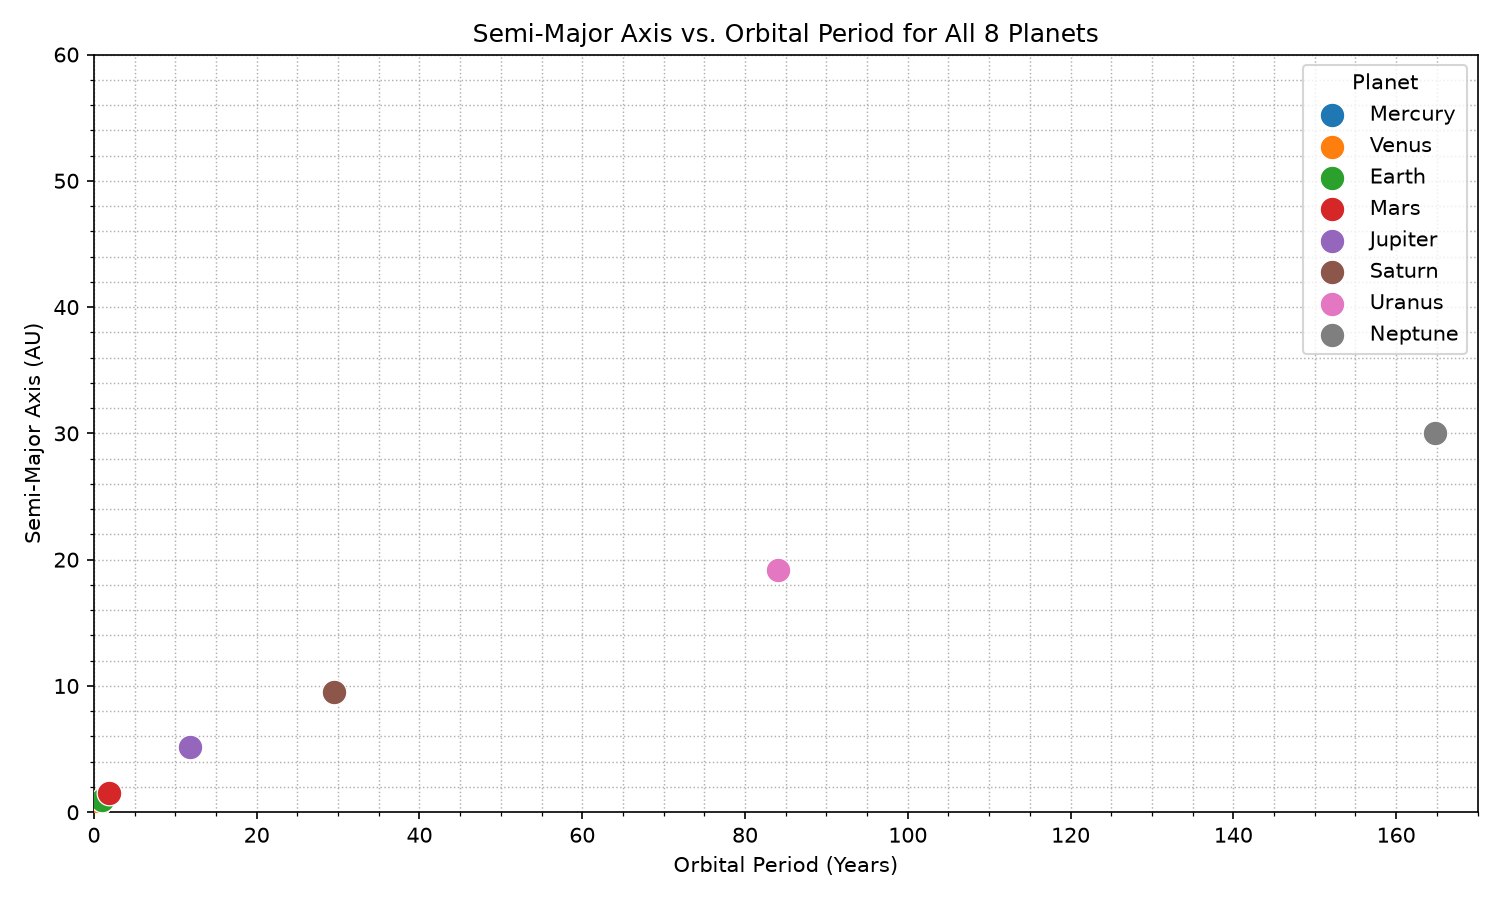
\includegraphics[width=0.95\linewidth]{Figures/math/all_planets_3.png}
    \caption{Period and semi major axis of all eight planets in our solar system.}
    \label{fig:all_planets}
\end{figure}

\textcolor{maincolor}{\textbf{\faPen\ f) Draw your best model $\hat{y}=cx$ (the straight line with the slope you found) in \cref{fig:all_planets}.}}

\question[3cm]{Look at your line together with the four outer planets. Judging by eye, does your model describe the outer planets well?}

\begin{solution}
The line shoots up far above the outer planets: it strongly overestimates their semi major axis. By eye, the linear model clearly fails outside the range of the training data.
\end{solution}

Let us now put a number on this. \Cref{tab:eight-planets} summarises the exact data for all eight planets. The four inner planets are the training data, while the four outer planets are the testing data.

\begin{table}[H]
\centering
\caption{Orbital periods and semi-major axes of the eight planets in the Solar System.}
\label{tab:eight-planets}
\begin{tabular}{|c|c|c|c|}
\hline
Planet & Orbital period (years) & Semi-major axis (AU) & Data use \\ \hline
Mercury & 0.240847 & 0.387099 & Training \\ \hline
Venus & 0.615197 & 0.723332 & Training \\ \hline
Earth & 1.000017 & 1.000000 & Training \\ \hline
Mars & 1.880816 & 1.523662 & Training \\ \hline
Jupiter & 11.862615 & 5.203363 & Testing \\ \hline
Saturn & 29.447498 & 9.537070 & Testing \\ \hline
Uranus & 84.016846 & 19.191264 & Testing \\ \hline
Neptune & 164.791320 & 30.068963 & Testing \\ \hline
\end{tabular}
\end{table}

\textcolor{maincolor}{\textbf{\faPen\ g) Use your own best model $\hat{y}=cx$ (with the value of $c$ that you found) to predict the semi major axis of each outer planet, and compute the $MSE$ on this testing data.}}

\calcspace[5cm]

\answerbox{$MSE_{\text{test}} ={}$}

\begin{solution}
Students use their own value of $c$, so the exact number will vary; the teacher can check the computation. For the optimal value $c = 0.885$, the result is $MSE_{\text{test}} \approx 4192$, which is enormous compared with the training error of $0.024$. The straight line that fitted the inner planets so nicely completely fails for the outer planets.
\end{solution}

\question{Do you think a linear model is suited to describe this data? Why (not)?}

\question[3cm]{What are the advantages and disadvantages of using \emph{all} of your data to build the model, versus keeping some data apart to test it at the end?}



\section{Fitting functions}\label{sec:fitting}

In the previous section, you found the best possible \emph{straight line} through the data and saw that it fails badly for the outer planets. Perhaps the relationship between period and distance is simply not linear, and a function with a different shape, namely a curve, describes the data better.

To find out, we could try many different models and, for each one, compute the loss ($MSE$) as we did before. But doing this by hand, over and over, is a lot of work. This is exactly the kind of repetitive calculation that a computer does well. From here on we let Python fit the models and compute the loss for us.

We will compare three types of model:
\begin{itemize}
  \item a \textbf{linear} model, \quad $a = c\,T$ \quad (a straight line through the origin, as in Section~\ref{sec:linreg});
  \item a \textbf{quadratic} model, \quad $a = \alpha\,T^2 + \beta\,T + \gamma$ \quad (a parabola);
  \item a \textbf{power-law} model, \quad $a = C\,T^{\,p}$ \quad (a curve whose steepness is set by the exponent $p$).
\end{itemize}

\begin{importantbox}
\textbf{Choose one of the following two ways to complete this part:}
\begin{itemize}
  \item \textbf{Option A: Guided notebook.} Open \textbf{``Fitting and machine learning''}. This notebook is ready to run: it loads the data, reproduces the linear fit you made by hand, and fits all three models, printing the loss ($MSE$) of each. Run the cells one by one and read what happens.
  \item \textbf{Option B: Write it yourself with AI.} Open \textbf{``Fitting and machine learning: AI version''}. Here, only the data is given. For each model, write the Python code yourself with the help of an AI language model (LLM). Ask it to plot the data and fit the linear, quadratic, and power-law models; then run its code and check that the result makes sense.
\end{itemize}
Whichever option you choose, answer the questions below.
\end{importantbox}

\question[2cm]{The notebook first reproduces the linear fit through the four inner planets. Which value of $c$ does it find, and does it agree with the value you found by hand in Section~\ref{sec:linreg}?}

\begin{solution}
The notebook finds $c \approx 0.885$, exactly the value the students found by hand (training $MSE \approx 0.024$, testing $MSE \approx 4192$).
\end{solution}

\question[1cm]{Run the fits of the three models on all eight planets, and write the loss ($MSE$) of each model in the table. Which model has the lowest loss?}

\vspace{0.3cm}
\begin{tabular}{|l|c|}
\hline
    Model & $MSE$ \\ \hline
    Linear \; $a=c\,T$ & \\ \hline
    Quadratic \; $a=\alpha T^2+\beta T+\gamma$ & \\ \hline
    Power law \; $a=C\,T^{p}$ & \\ \hline
\end{tabular}
\vspace{0.3cm}

\begin{solution}
Linear $MSE \approx 4.66$; quadratic $MSE \approx 0.39$; power law $MSE \approx 0$ (about $10^{-6}$). The power law has by far the lowest loss.
\end{solution}

\question[2cm]{Look at the plots of the fitted models. Which model follows the data points best across the \emph{whole} range, from Mercury to Neptune?}

\begin{solution}
The power law. On logarithmic axes, it is a perfectly straight line passing through every planet; the quadratic drifts away at small periods, and the straight line is far too low for the outer planets.
\end{solution}

\question[2cm]{The power-law model is $a = C\,T^{p}$. What values did the fit find for $C$ and for the exponent $p$? Keep the exponent in mind because we will return to it later.}

\begin{solution}
$C \approx 1$ and $p \approx 0.667 \approx \tfrac{2}{3}$, so the data follow $a \approx T^{2/3}$. This is Kepler's third law in disguise (Section~\ref{sec:kepler}).
\end{solution}

\question[3cm]{Why is it useful to try several different models, instead of just picking one and hoping it is right?} 

\question[3cm]{Why can the power law, with only two parameters, beat the quadratic, which has three?}

\begin{solution}
We do not know the true relation in advance, so we let the data decide by comparing the loss of several candidate models. A model with the \emph{right shape} (the power law) can fit far better than a more flexible model with more parameters but the wrong shape (the quadratic): more parameters do not help if the form of the function is wrong.
\end{solution}

\question[4cm]{\emph{(Option B only.)} Which instructions, or ``prompts'', did you give the AI to obtain the code? Did the code work the first time, or did you have to correct it? How did you check that the result was actually right?}

\begin{solution}
Discussion question. The key point is that an AI can write code quickly, but \emph{you} remain responsible for checking that it does the right thing. You must read and run the code, then judge whether the numbers and plots make sense. This is the same critical attitude we need towards any model or tool.
\end{solution}

\section{Neural networks}\label{sec:nn}

In the previous section, you chose a \emph{formula} for your model, such as a line, a parabola, or a power law, and then adjusted its few parameters to make the loss small. \emph{Machine learning} takes a similar approach: instead of choosing a formula, we use a very flexible model with \emph{many} parameters and let the computer adjust all of them automatically to make the loss small.

The best-known model of this type is the \emph{neural network}. A simplified example is shown in \cref{fig:neural-network}. It is built from many small units (``neurons'') connected by adjustable parameters called \emph{weights}. Each choice of weights produces a different function and therefore different predictions.

\begin{importantbox}
\textbf{Training a neural network is still function fitting.} In Section~\ref{sec:linreg}, your model was the function $\hat{y}=cx$. You adjusted the parameter $c$ to make the loss as small as possible. A neural network follows exactly the same principle, but its function contains many adjustable weights instead of one parameter. The computer makes predictions, calculates the loss, changes the weights to reduce the loss, and repeats this process. This repeated minimisation of the loss function is called \emph{training}. Gradient descent tells the computer how to adjust the weights at each step.
\end{importantbox}

\begin{figure}[H]
    \centering
    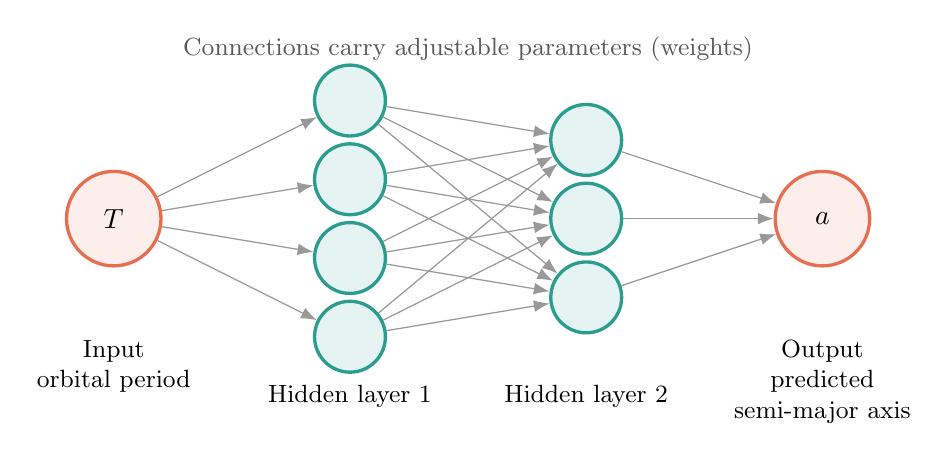
\begin{tikzpicture}[
        neuron/.style={circle, draw=maincolor, very thick, fill=maincolor!12, minimum size=9mm, inner sep=0pt},
        endpoint/.style={circle, draw=accentcolor, very thick, fill=accentcolor!12, minimum size=12mm, inner sep=0pt},
        connection/.style={draw=black!40, line width=0.45pt, -{Latex[length=2mm]}},
        layerlabel/.style={align=center, font=\small}
    ]
        \node[endpoint] (input) at (0,0) {$T$};

        \foreach \i/\y in {1/1.5,2/0.5,3/-0.5,4/-1.5}
            \node[neuron] (hiddenone\i) at (3,\y) {};

        \foreach \i/\y in {1/1,2/0,3/-1}
            \node[neuron] (hiddentwo\i) at (6,\y) {};

        \node[endpoint] (output) at (9,0) {$a$};

        \foreach \i in {1,...,4}
            \draw[connection] (input) -- (hiddenone\i);

        \foreach \i in {1,...,4}
            \foreach \j in {1,...,3}
                \draw[connection] (hiddenone\i) -- (hiddentwo\j);

        \foreach \j in {1,...,3}
            \draw[connection] (hiddentwo\j) -- (output);

        \node[layerlabel, below=8mm of input] {Input\\orbital period};
        \node[layerlabel] at (3,-2.25) {Hidden layer 1};
        \node[layerlabel] at (6,-2.25) {Hidden layer 2};
        \node[layerlabel, below=8mm of output] {Output\\predicted\\semi-major axis};

        \node[font=\small, text=black!65] at (4.5,2.15) {Connections carry adjustable parameters (weights)};
    \end{tikzpicture}
    \caption{A simplified neural network that uses the orbital period $T$ to predict the semi-major axis $a$. During training, the network adjusts the parameters of the connections to reduce the loss function.}
    \label{fig:neural-network}
\end{figure}

\subsection*{Why gradient descent is needed}

For the linear model $\hat{y}=cx$, the loss $MSE(c)$ was a simple function of one parameter. In Route~2, you differentiated this function, set the derivative equal to zero, and solved an equation to find the minimum exactly.

The loss of a neural network is also a mathematical function, but it depends on many weights at the same time:
\[
    L=L(w_1,w_2,\ldots,w_k).
\]
This function has derivatives, but it is usually far too complicated to solve all the equations for the global minimum exactly. Instead, the computer calculates the \emph{local gradient}: the derivatives of the loss at the current values of the weights. The gradient shows the direction in which the loss increases most quickly, so moving a small step in the opposite direction should lower the loss.

The computer then calculates the gradient again at the new point and takes another small step. This process combines the derivative information from Route~2 with the repeated improvements from Route~1. Repeating these local steps is called \emph{gradient descent}, as illustrated in \cref{fig:gradient-descent}.

\begin{figure}[H]
    \centering
    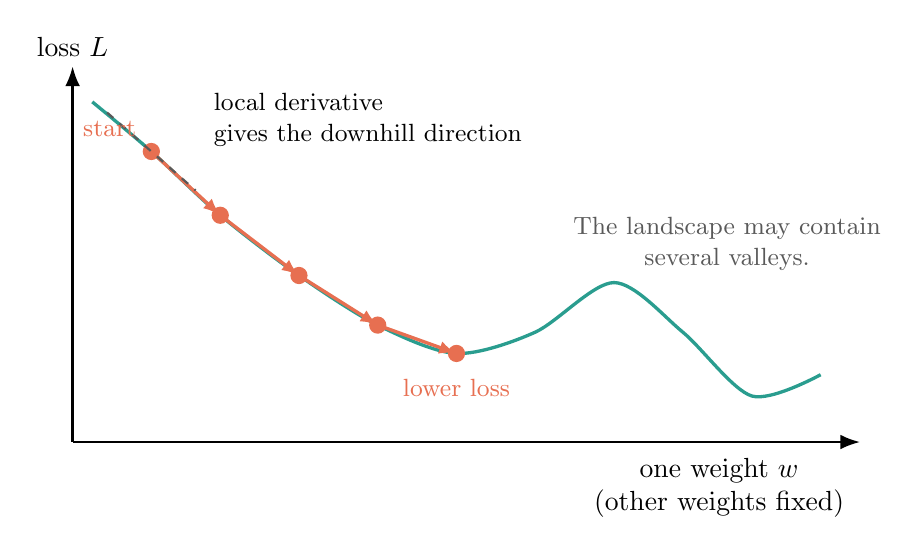
\begin{tikzpicture}[
        x=1.25cm,
        y=0.9cm,
        gdarrow/.style={-{Latex[length=2.2mm]}, very thick, accentcolor},
        point/.style={circle, fill=accentcolor, inner sep=2.2pt}
    ]
        \draw[-{Latex[length=2.5mm]}, thick] (0,0) -- (8,0)
            node[below left=1mm, align=center] {one weight $w$\\(other weights fixed)};
        \draw[-{Latex[length=2.5mm]}, thick] (0,0) -- (0,5.3)
            node[above] {loss $L$};

        \draw[maincolor, very thick, smooth]
            plot coordinates {(0.2,4.8) (0.8,4.1) (1.5,3.2) (2.3,2.35)
                              (3.1,1.65) (3.9,1.25) (4.7,1.55) (5.5,2.25)
                              (6.2,1.55) (6.9,0.65) (7.6,0.95)};

        \coordinate (pzero) at (0.8,4.1);
        \coordinate (pone) at (1.5,3.2);
        \coordinate (ptwo) at (2.3,2.35);
        \coordinate (pthree) at (3.1,1.65);
        \coordinate (pfour) at (3.9,1.25);

        \draw[gdarrow] (pzero) -- (pone);
        \draw[gdarrow] (pone) -- (ptwo);
        \draw[gdarrow] (ptwo) -- (pthree);
        \draw[gdarrow] (pthree) -- (pfour);

        \node[point] at (pzero) {};
        \node[point] at (pone) {};
        \node[point] at (ptwo) {};
        \node[point] at (pthree) {};
        \node[point] at (pfour) {};

        \draw[black!65, dashed, thick] (0.35,4.65) -- (1.25,3.55);
        \node[align=left, font=\small] at (3.0,4.55)
            {local derivative\\gives the downhill direction};

        \node[font=\small, accentcolor, above left=1mm] at (pzero) {start};
        \node[font=\small, accentcolor, below=2mm] at (pfour) {lower loss};
        \node[font=\small, align=center, text=black!65] at (6.65,2.8)
            {The landscape may contain\\several valleys.};
    \end{tikzpicture}
    \caption{Gradient descent on a one-dimensional slice of a loss landscape. At each point, the local derivative determines the downhill direction. After a small step, the derivative is calculated again. A real neural network has many weights, so its loss landscape has many dimensions.}
    \label{fig:gradient-descent}
\end{figure}




\question[3cm]{In Section~\ref{sec:linreg} you tuned a single parameter $c$ by hand. A neural network can have thousands of parameters. Why is it impossible to tune these by hand, and what do we need instead?}

\begin{solution}
By hand, we can adjust only one or two numbers at a time. With thousands of parameters, this would be impractical, so we need a computer to carry out an automatic procedure called gradient descent.
\end{solution}

\question[3cm]{A neural network can fit almost any shape. Can you think of an advantage \emph{and} a possible disadvantage of using such a very flexible model?}

\begin{solution}
Its advantage is that it can model relationships even when we do not know which formula to use. Its disadvantages are that it has many difficult-to-interpret parameters, can fit noise, and does not provide a simple, understandable law, as we are about to see.
\end{solution}

\section{Working with neural network models}\label{sec:nnwork}

How  good would a neural network be in predicting the semi-major axis from the orbital period? Let us now train a neural network on our planet data, and see how it compares with the models you have already tried.

\begin{importantbox}
\textbf{Choose one of the following two ways to complete this part:}
\begin{itemize}
  \item \textbf{Option A: Guided notebook.} Open \textbf{``Neural network''}. This notebook is ready to run: it loads the data, trains a small neural network to predict the semi-major axis from the period, plots the fit, and compares it with the power law from Section~\ref{sec:fitting}. At the end, there are extensions to try, such as larger networks and other activation functions.
  \item \textbf{Option B: Write it yourself with AI.} Open \textbf{``Neural network: AI version''}. Here, only the data is given. Build and train the network yourself with the help of an AI language model (LLM). Ask it to scale the data, build and train the network, plot the fit, and compare it with the power law; then run its code and check the result.
\end{itemize}
Whichever option you choose, answer the questions below.
\end{importantbox}

\question[2cm]{Does the neural network manage to follow the data? Write down its loss ($MSE$), and compare it with the loss of the power-law model from Section~\ref{sec:fitting}.}

\begin{solution}
The network follows the data well (its $MSE$ is small, about $0.01$). The power law is still a little better (its $MSE$ is essentially $0$, about $10^{-6}$).
\end{solution}

\question[2cm]{How many parameters (weights) does the neural network use, and how many does the power law use? Which model is simpler?}

\begin{solution}
The small network uses about $25$ weights; the power law uses only $2$ parameters. The power law is far simpler and fits at least as well.
\end{solution}

\question[3cm]{In the extensions you tried larger networks and different activation functions. Did a bigger network always give a lower loss? Which activation followed the data best?}

\begin{solution}
No. With only eight data points, a larger network does not reliably fit better because it has more weights but no additional data to determine them. The smooth activation functions (\texttt{tanh} and \texttt{logistic}) follow the smooth planetary curve better than \texttt{relu}, which produces straight segments with sharp changes in direction.
\end{solution}

\question[4cm]{Both the power law and the neural network fit the eight planets well. If you had to predict the orbit of a completely new planet, far outside the range of our data, which model would you trust more, and why?}

\begin{solution}
The power law: it has the right shape and captures the underlying law, so it extrapolates sensibly. The neural network gives no guarantee outside the range of its training data and can behave in strange ways there.
\end{solution}

\question[3cm]{Which of the two models provides an interpretable relationship that helps you \emph{understand} nature, and which is a ``black box'' of numbers?}

\begin{solution}
The power law is interpretable: its exponent $\tfrac{2}{3}$ is a real physical law (Section~\ref{sec:kepler}). The neural network is a black box: its $25$ weights carry no simple meaning.
\end{solution}

\question[4cm]{\emph{(Option B only.)} Which prompts did you give the AI to build and train the network? Did its code work the first time? How did you check that the network's result was sensible?}

\begin{solution}
Discussion question. As in Section~\ref{sec:fitting}, the point is that the AI can write the code quickly, but you stay responsible for reading it, running it, and judging whether the fit and the numbers make sense.
\end{solution}

\subsection*{When is a neural network the better choice?}

For our planet problem, the interpretable power law beat the neural network: we had only a few data points, and there was a clean underlying law. But this is not always the case. Neural networks work well when there is a \emph{lot} of data and \emph{no} simple formula to be found.

A striking example comes from the search for exoplanets itself. Recall from the introduction that a planet passing in front of its star makes the star's brightness dip a little; the record of the brightness over time is called a \emph{light curve} (\cref{fig:transit}). Space telescopes such as Kepler and TESS measured the light curves of \emph{hundreds of thousands} of stars.

\begin{figure}[htbp]
    \centering
    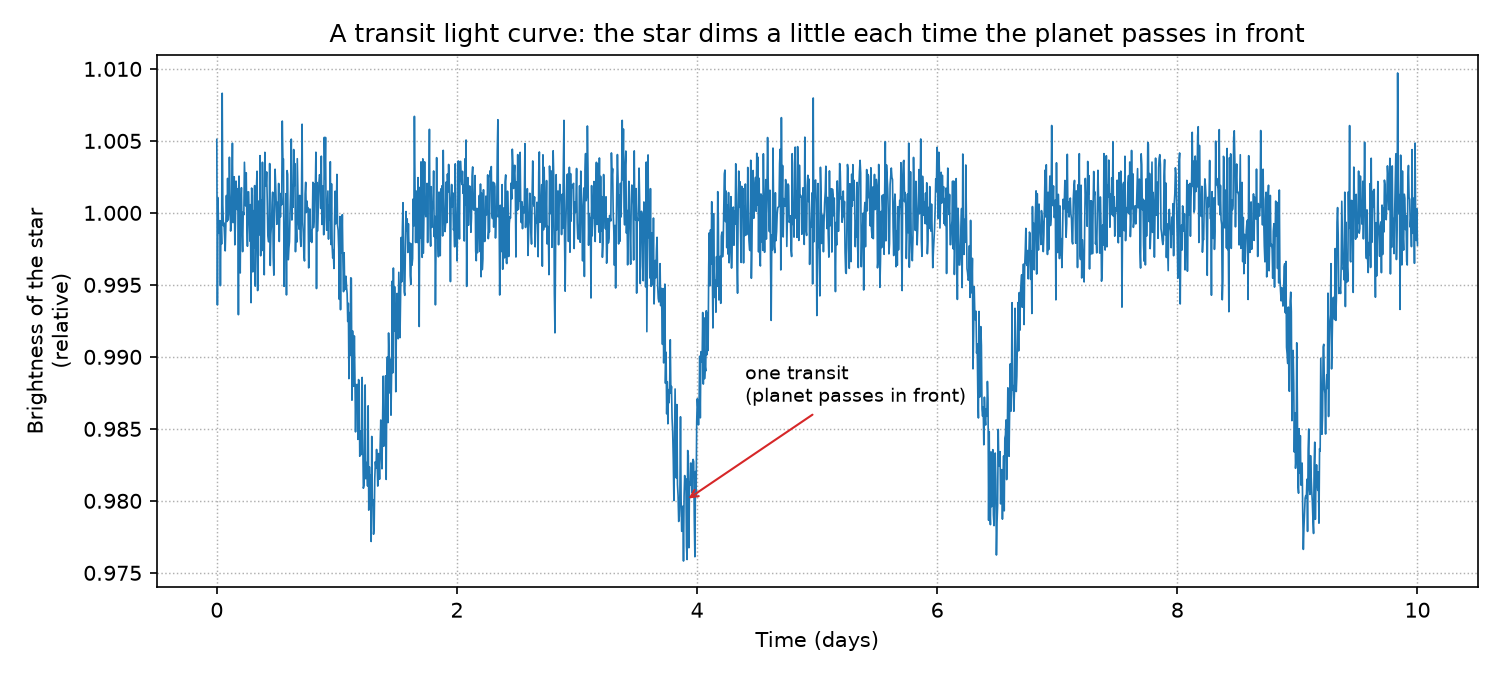
\includegraphics[width=0.9\linewidth]{Figures/math/transit_lightcurve.png}
    \caption{A transit light curve: each time the planet passes in front of its star, the measured brightness dips a little. Real data are noisy, and most dips are not caused by planets.}
    \label{fig:transit}
\end{figure}

The catch is that most dips are \emph{not} planets. Pairs of stars eclipsing each other, dark spots on a star's surface, and instrument noise all produce look-alike signals. There is no neat formula that separates a real planet from a false alarm, and there are far too many candidates to check by hand. This is the opposite of the situation with Kepler's law: an enormous amount of data, and no simple model.

This is exactly where neural networks shine. In 2018, researchers trained a neural network on thousands of labelled Kepler light curves. It learned to recognise real transits and even found a planet that people had missed, Kepler-90\,i. This discovery made Kepler-90 the first star besides our Sun known to have \emph{eight} planets.\footnote{C.~J. Shallue \& A.~Vanderburg, \emph{Astronomical Journal} \textbf{155}, 94 (2018); the network is known as \emph{AstroNet}.} In 2021, NASA's \emph{ExoMiner} network validated 301 new exoplanets at once, more reliably than earlier software or human experts, and its successor now scans data from the TESS telescope.\footnote{H.~Valizadegan et al., \emph{Astrophysical Journal} \textbf{926}, 120 (2022); the open-source \emph{ExoMiner++} (2026) analyses TESS data. See also \href{https://science.nasa.gov/universe/exoplanets/new-deep-learning-method-adds-301-planets-to-keplers-total-count/}{NASA Science}.}

\question[6cm]{For each of the two tasks below, would you choose an interpretable model or a flexible neural network, and why? \; (a)~estimating a planet's radius from the transit depth when the radius of its star is known; \; (b)~screening thousands of noisy atmospheric spectra to identify which ones may contain signs of water vapour.}

\begin{solution}

(a)~An interpretable model. Transit depth and the radii of the planet and star are connected by a simple geometric relationship. A formula is therefore more transparent and useful than a neural network.

(b)~A neural network. Atmospheric spectra contain many wavelengths, overlapping signals, and noise. If many labelled examples are available, a flexible model can learn complicated patterns that would be difficult to describe with one simple formula.

\textbf{The rule of thumb:} use a simple, interpretable model when you want to \emph{understand} a law from limited data; reach for a neural network when you have \emph{lots} of data and no known formula.
\end{solution}


\vspace{0.5cm}
\textcolor{accentcolor}{\textbf{\faLightbulb\ Closing the challenge}}

\section{Discover Kepler's Law}\label{sec:kepler}

In Section~\ref{sec:fitting} you found that the power-law model $a = C\,T^{p}$ fits the planet data almost perfectly, with
$$C \approx 1 \qquad\text{and}\qquad p \approx 0.667.$$
A neural network could also fit the data, but it hid the relationship inside many weights. The power law, by contrast, is simple enough to \emph{read}. Let us now turn this fitted model into a physical law.

\question[2cm]{The exponent $p \approx 0.667$ is very close to a simple fraction. Which fraction is it? Using $C \approx 1$, write down the resulting relation between $a$ and $T$.}

\begin{solution}
$p \approx \tfrac{2}{3}$, so $a \approx T^{2/3}$.
\end{solution}

\question[3cm]{Rewrite the relation $a = T^{2/3}$ without a fractional exponent, by raising both sides to the power $3$. What equation do you get?}

\begin{solution}
$$\left(a\right)^3 = \left(T^{2/3}\right)^3 \quad\Longrightarrow\quad a^3 = T^2.$$
\end{solution}

\begin{importantbox}
Congratulations! You have just rediscovered \textbf{Kepler's third law}:
$$T^2 = a^3,$$
where $T$ is the orbital period in years and $a$ is the semi major axis in AU. In words: \emph{the square of the orbital period equals the cube of the semi major axis.} It took Johannes Kepler about ten years to extract this law from Tycho Brahe's observations; you found it from the data in a single afternoon.
\end{importantbox}

The clean form $T^2 = a^3$ appears because we measured $T$ in years and $a$ in AU. These units are defined relative to Earth's orbit, for which $T = 1$ and $a = 1$. In other units, the law reads $T^2 \propto a^3$. Newton later showed \emph{why} it holds: it follows from his law of gravity, and the full form is
$$T^2 = \frac{4\pi^2}{G\,M}\,a^3,$$
where $M$ is the mass of the star and $G$ is the gravitational constant. For a star with a different mass from the Sun, the constant changes. We will need this result in the next section.

\question[3cm]{Check the law: use $a = T^{2/3}$ to predict the semi-major axis of Saturn, whose orbital period is $T = 29.45$ years. Compare your answer with the measured value in \cref{tab:eight-planets}.}

\begin{solution}
$a = 29.45^{2/3} \approx 9.54$ AU, in excellent agreement with the measured value.
\end{solution}

\question[3cm]{We now have two things that both describe the data well: a neural network, and the simple law $T^2 = a^3$. Which of the two would you call a \emph{law of nature}, and why?}

\begin{solution}
The simple law $T^2 = a^3$: it is exact, has no free parameters left, applies to every planet, and can be understood and explained (through gravity). The neural network only reproduces the data numerically, without revealing any such law.
\end{solution}

\question[3cm]{Kepler found this law purely from data, long before Newton explained it with gravity. Does finding a pattern in data always mean that we understand \emph{why} it is true?}

\begin{solution}
No. A fitted relationship \emph{describes} the data but does not, by itself, \emph{explain} the cause. Kepler had the correct pattern but the wrong explanation because he imagined magnetic fibres extending from the Sun. The real explanation, gravity, came later with Newton. Finding a pattern, whether through curve fitting or a neural network, is only the first step; understanding the mechanism is another.
\end{solution}

Now that we have Kepler's law, we can rearrange it. If we measure a planet's orbital period, we can \emph{compute} its distance from the star, represented by its semi-major axis. In the next section, you will do exactly this for your own exoplanet.



\section{Applying it to your own exoplanet}\label{sec:exoplanet}

At the beginning of the lesson, we set you a challenge: find the distance between your exoplanet and its star. You now have everything you need: a way to measure the period from a transit light curve and Kepler's law to convert that period into a distance.

There is one extra ingredient. The law $T^2 = a^3$ holds for planets orbiting the \emph{Sun}. Your exoplanet orbits a different star, with a different mass $M$. As we saw in the previous section, Newton's version of the law then becomes, when we measure the period $T$ in years, the semi major axis $a$ in AU, and the star's mass $M$ in solar masses ($M_\odot$):
$$T^2 = \frac{a^3}{M}, \qquad\text{which we can solve for the distance:}\qquad a = \sqrt[3]{M\,T^2}.$$
For a star with the same mass as the Sun ($M = 1$) this is exactly the law you rediscovered.

\begin{promptbox}
\textbf{Worked example.} A planet with period $T = 2$ years, orbiting a star of mass $M = 1.2\,M_\odot$, has
$$a = \sqrt[3]{1.2 \times 2^2} = \sqrt[3]{4.8} \approx 1.69 \text{ AU},$$
so it orbits a little farther from its star than the Earth does from the Sun. \emph{(A cube root is the same as raising to the power $\tfrac{1}{3}$ on your calculator.)}
\end{promptbox}

\vspace{0.5cm}
\textbf{Step 1: Find the period $T$.} Your data sheet contains a transit light curve of your exoplanet. It shows the brightness of the star over time, with a dip each time the planet passes in front of it. The time between two consecutive dips is one orbital period.

\textcolor{maincolor}{\textbf{\faPen\ Read the period $T$ of your exoplanet from your transit light curve.}} To be more accurate, measure the total time across \emph{several} transits and divide by the number of periods in between.

\answerbox[4cm]{$T ={}$} years.
(Add the value of $T$ to your planet factsheet.)

\vspace{0.5cm}
\textbf{Step 2: Write down your star's mass $M$.} You can find the mass of your exoplanet's host star on your data sheet.

\answerbox[4cm]{$M ={}$} solar masses ($M_\odot$)

\vspace{0.5cm}
\textbf{Step 3: Compute the distance $a$.} Substitute your values of $T$ and $M$ into the formula $a = \sqrt[3]{M\,T^2}$.

\calcspace[4cm]

\answerbox[4cm]{$a ={}$} AU.
(Add the value of $a$ to your planet factsheet.)

\vspace{0.5cm}
\textbf{Step 4: Interpret your result.}

\question[3cm]{Is your exoplanet closer to or farther from its star than the Earth is from the Sun? Is there a planet in our solar system that has a similar distance?}

\question[3cm]{This week, you are gathering different pieces of information about your mystery planet. Now that you know its distance from its star, what might that tell you about the planet? For example, what could you infer about its temperature or whether it could have liquid water?}

\begin{solution}
Open discussion, linking to the other lessons of the week. The distance to the star strongly affects how much light and heat the planet receives: too close and it is scorching, too far and it is frozen; only a narrow range of distances (the ``habitable zone'') allows liquid water. The exact zone also depends on how bright the star is.
\end{solution}

\begin{importantbox}
\textbf{Well done! Challenge complete.} Starting with only a table of numbers, you have followed in Kepler's footsteps: you fitted models, measured their loss, explored neural networks and machine learning, rediscovered Kepler's third law, and used it to find the distance between your exoplanet and its star.
\end{importantbox}






\vspace{0.5cm}
\textcolor{accentcolor}{\textbf{\faLightbulb\ What have we learned?}}

\question{What have you learned that you didn't know before?}

\question{How have you used AI in this lesson, and what did you learn from it?}





















\end{document}